DOGS is an extension of the DOG system. The first 3 letters can be directly translated from danish to \textit{dynamic optimization of greens} and the appended S of the herein regarded system means \textit{coordination}. Thus DOG is an traffic actuated optimizer for single intersections, as described in section \ref{actuated}, and DOGS add coordination.

DOGS is a criteria-based system which relies on a common cycle time for coordination. The intended area of application is traffic signals along arterials, which see a high fluctuation of demand. 

The Danish Road Directorate (DRD) has implemented DOGS along several arterials in Denmark. 
Among these are the Glostrup and Herlev implementations along the O3 ring-road. They see high increases in demand in the morning and afternoons when commuters come to and leave work places. Normally such fluctuations can be handled well by a fixed number of timing plans (see section \ref{pretimed}), which are changed according to the time of day, but the area also see more unpredictable types of fluctuations when accidents occur on the nearby highway, M3, or when M3 lanes are closed due to expansions. For these reasons DRD decided implement a system which could handle such situations.

The purpose of DOGS is to increase the capacity of the arterial in these cases - in low traffic situations pretimed plans will be used. The capacity increase comes by adjusting a common cycle time and thus allocating more green time to the major phases. This will cause increased delays for the minor roads, but may prevent queues from reaching the previous intersection - or even prevent queues in cases of light congestion.
DOGS is also capable of providing priority to buses by extending the green time when buses are near an intersection.

At present the system must be tailored to the environment in which is must operate. For this reason the following sections will use the Herlev area as a reference area in order to explain certain concepts. In figure \ref{fig:dogs_herlev} is a layout of this network.

\begin{figure}[!ht]
\begin{center}
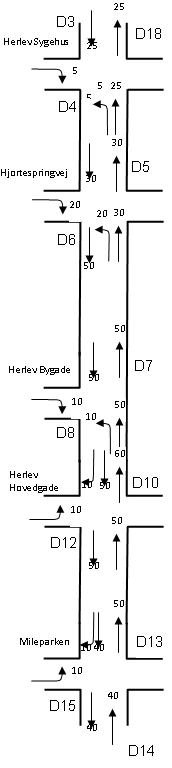
\includegraphics[scale=0.5]{dogs_herlev.png} 
\end{center}
\caption{Layout of the partial O3 arterial in Herlev, which is under DOGS control. The arrows and numbers indicate flow direction and indications of vehicle count.}
\label{fig:dogs_herlev}
\end{figure}

\subsubsection*{Detection}
Loops are placed in the immediate downstream of signal controllers and connected to closest controller to reduce the wire length. 

The criteria which DOGS use are based on the load on the detectors and the number of vehicles detected per cycle. Furthermore the detectors are capable of measuring vehicle speeds, though this is not taken into consideration in any of the criteria.

\subsubsection*{Prediction}
DOGS is a purely traffic actuated system and no prediction is used when the system is activated due to heavy traffic conditions.

In spite of the flexibility of the system this is a point which puts high demand on the implementing traffic engineers since traffic through the arterial must be assessed manually when the system is put into production as well as during maintenance.

\subsubsection*{Optimization}
Since DOGS only kicks in under congested or near-congested conditions (for the Herlev area when the load exceeds 60\%) it is simple to optimize the throughput since, as explained earlier, any increase in green time will just allow more vehicles to pass (the phase is never emptied from vehicles).

The load measurement in Herlev is extracted from detectors, which are strategically placed in the ends of the arterial. During an interview with DRD and TTS it was explained that the traffic from minor roads can be neglected in the load measurement, though both parties would be interested in seeing the effect of increasing the number of detectors used.

The common cycle time is set according to the load level and to avoid sudden, major changes in cycle time and temporary loss of coordination, cycle time and green times are adjusted to within some maximum per cycle. 

Coordination is achieved by running the signals on the common cycle time, but offsets are not adjusted when the common cycle time changes so this issue should receive further investigation.